%%%%%%%%%%%%%%%%%%%%%%%%%%%%%%%%%%%%%%%%%
% University/School Laboratory Report
% LaTeX Template
% Version 4.0 (March 21, 2022)
%
% This template originates from:
% https://www.LaTeXTemplates.com
%
% Authors:
% Vel (vel@latextemplates.com)
% Linux and Unix Users Group at Virginia Tech Wiki
%
% Eddited by:
% Johann Becker, Valentin Eder, Marc Ostner
%
% License:
% CC BY-NC-SA 4.0 (https://creativecommons.org/licenses/by-nc-sa/4.0/)
%
%%%%%%%%%%%%%%%%%%%%%%%%%%%%%%%%%%%%%%%%%

%----------------------------------------------------------------------------------------
%	PACKAGES AND DOCUMENT CONFIGURATIONS
%----------------------------------------------------------------------------------------
\documentclass[
	a4paper, % Paper size, specify a4paper (A4) or letterpaper (US letter)
	12pt, % Default font size, specify 10pt, 11pt or 12pt
]{CSUniSchoolLabReport}

\usepackage[ngerman]{babel}
\usepackage{siunitx}  
\usepackage{textcase}
\usepackage{booktabs}
\usepackage[utf8]{inputenc}
\usepackage{amsmath}
\usepackage{array}
\usepackage{booktabs}
\usepackage{color}
\usepackage{tabularray}
\usepackage{pdfpages}

\sisetup{locale = DE,  
separate-uncertainty,  
range-units = brackets,  
list-units = single,  
per-mode=symbol-or-fraction,
}

\addbibresource{sample.bib} % Bibliography file (located in the same folder as the template)
\renewcommand{\thesection}{\Alph{section}}
\renewcommand{\thesubsection}{\thesection.\arabic{subsection}}
\renewcommand{\thesubsubsection}{\thesubsection.\arabic{subsubsection}}
\newcommand{\micro}{\ensuremath{\mu}}
\newcommand{\pico}{p}
\newcommand{\milli}{m}
\newcommand{\nano}{n}

%----------------------------------------------------------------------------------------
%	REPORT INFORMATION
%----------------------------------------------------------------------------------------
\setlength{\parindent}{0pt}

\title{Protokoll Praktikum EBau Diode} % Report title

\author{Johann \textsc{Becker} \and Valentin \textsc{Eder} \and Marc \textsc{Ostner}}
\date{\today} % Date of the report

%----------------------------------------------------------------------------------------

\begin{document}
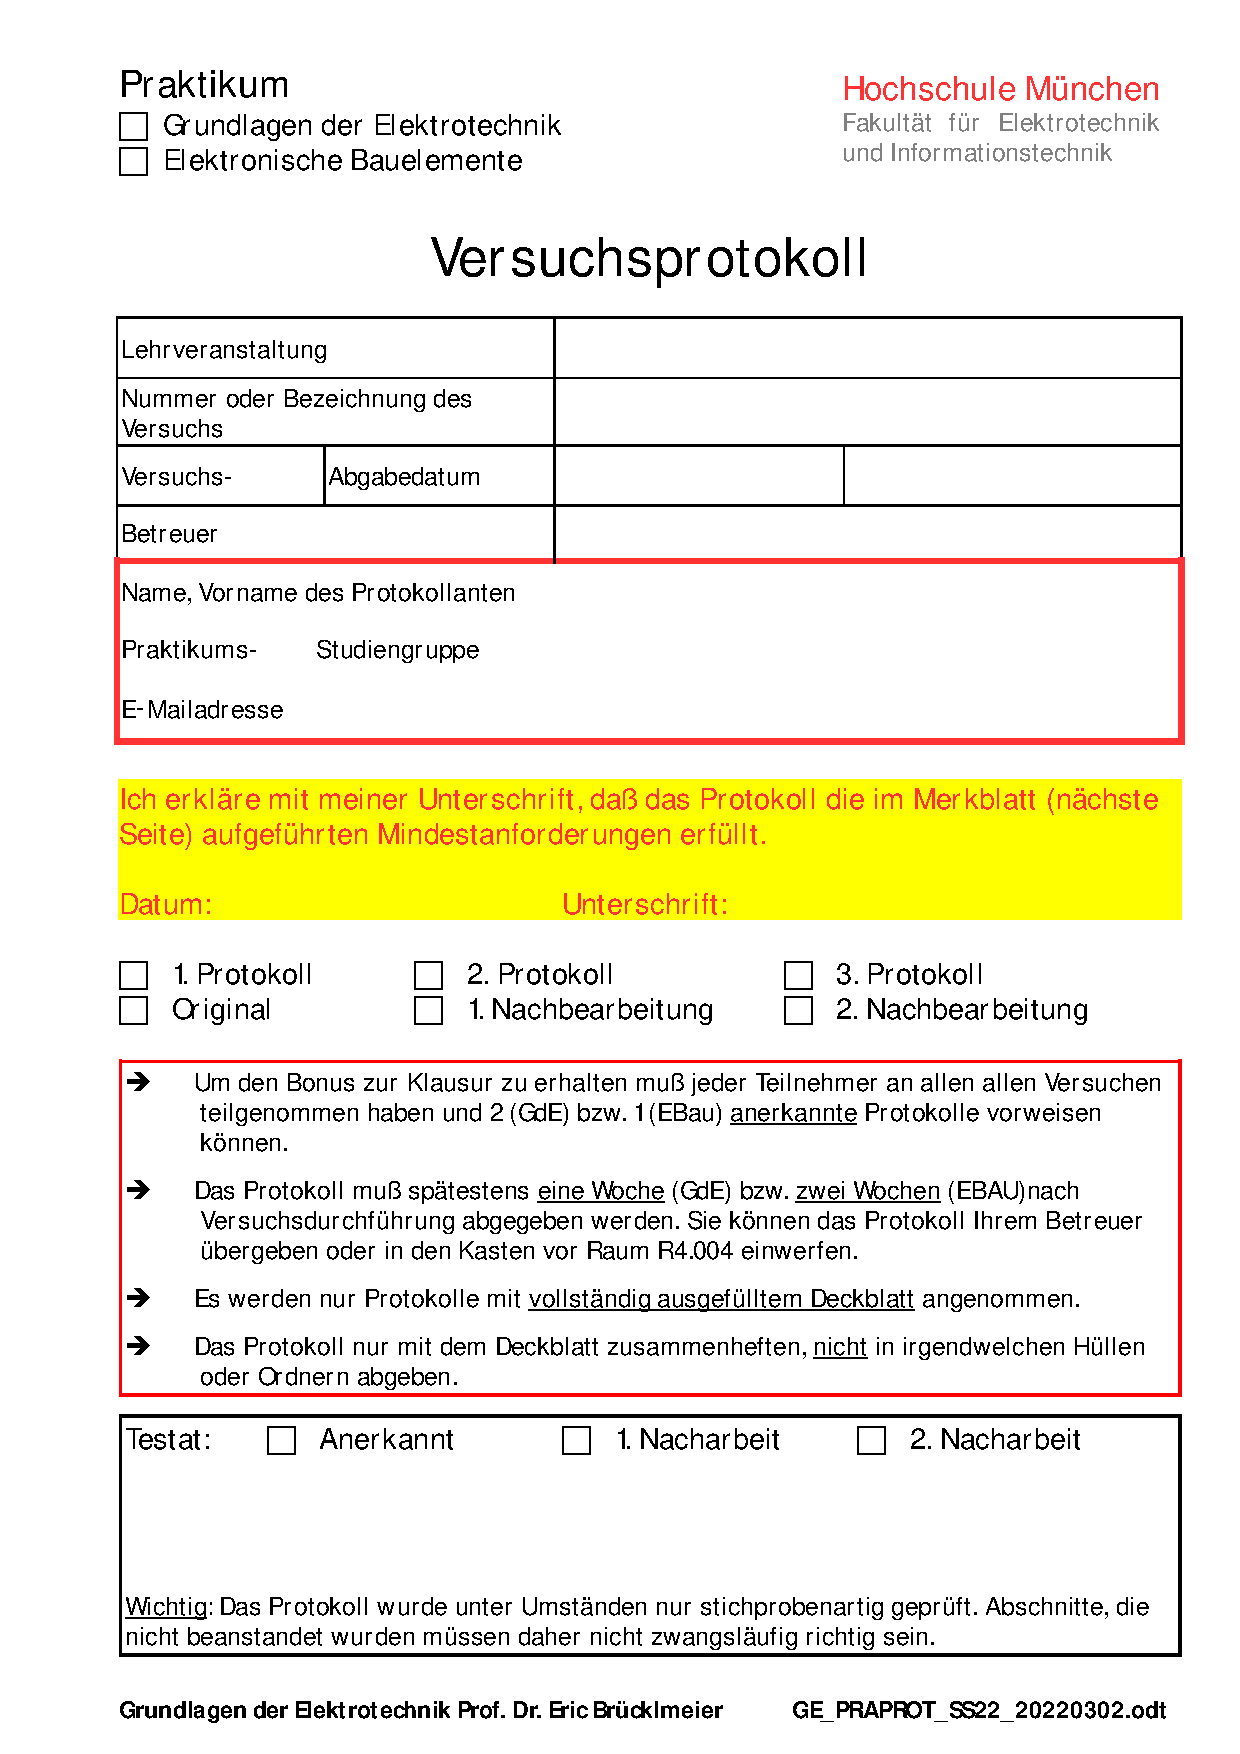
\includepdf{DeckblattEBAU.pdf}

\maketitle % Insert the title, author and date using the information specified above

\begin{center}
	\begin{tabular}{l r}
		Date Performed: & 30. Mai 2025 \\ % Date the experiment was performed
		
		Instructor: & Prof. Dr. Alexandru Negut % Instructor/supervisor
	\end{tabular}
\end{center}

%----------------------------------------------------------------------------------------
%	OBJECTIVE
%----------------------------------------------------------------------------------------

%A
\section{Einführung}
Die Vorbereitung ist im Anhang zu finden.

%B
\section{Versuchsdurchführung}

%B.1
\subsection{Statische Messungen}

%B.1.1
\subsubsection{Sperrschichtkapazität}

\begin{figure}[H] % [H] forces the figure to be placed exactly where it appears in the text
	\centering % Horizontally center the figure
	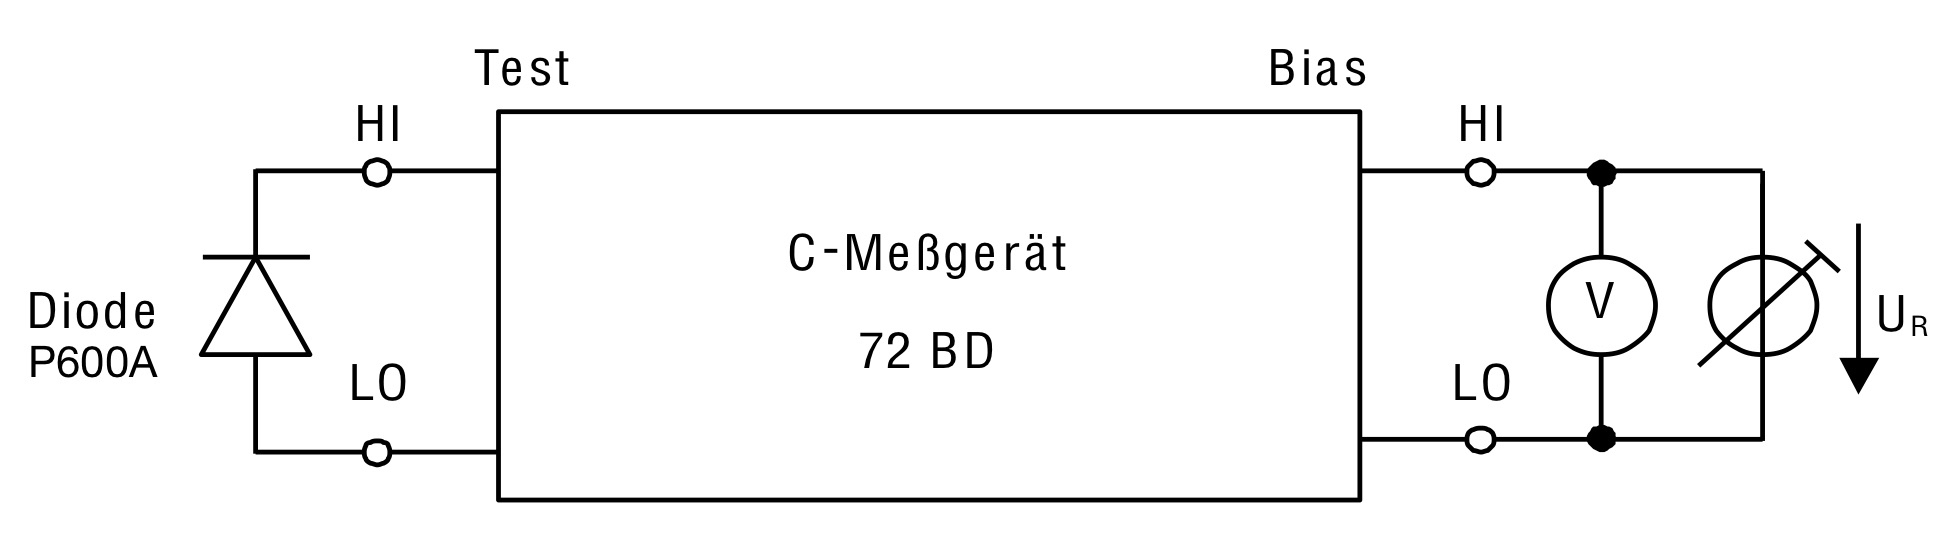
\includegraphics[width=0.7\textwidth]{B1.1 Versuchsaufbau} % Include the figure, now larger
	\caption{Versuchsaufbau für Messung der Sperrschichtkapazität}
\end{figure}

\begin{table}[ht]
\centering
\begin{longtblr}[
  label = none,
  entry = none,
]{
  width = \linewidth,
  colspec = {Q[129,c]Q[77,c]Q[119,c]Q[117,c]Q[119,c]Q[117,c]Q[77,c]Q[119,c]},
  vline{2} = {-}{},
  hline{2} = {-}{},
}
U/V  & 0     & 0,1   & 0,2   & 0,3  & 0,5  & 0,7  & 1    & 1,5  & 2  & 3,5  \\
C/pF & 122,6 & 110,1 & 102,4 & 96,5 & 87,8 & 81,6 & 74,8 & 67,2 & 62 & 52,5 
\end{longtblr}
\caption{Sperrschichtkapazitäten zwischen 0 bis \SI{3.5}{\volt}}
\end{table}

\begin{table}[ht]
\centering
\begin{longtblr}[
  label = none,
  entry = none,
]{
  width = \linewidth,
  colspec = {Q[129,c]Q[77,c]Q[119,c]Q[117,c]Q[119,c]Q[117,c]Q[77,c]Q[119,c]},
  vline{2} = {-}{},
  hline{2} = {-}{},
}
U/V  & 5  & 8    & 10   & 15   & 20   & 25 & 30   \\
C/pF & 47 & 40,5 & 37,7 & 33,1 & 30,1 & 28 & 26,4 
\end{longtblr}
\caption{Sperrschichtkapazitäten zwischen 3,5 bis \SI{30}{\volt}}

\end{table}

\begin{figure}[H] % [H] forces the figure to be placed exactly where it appears in the text
	\centering
	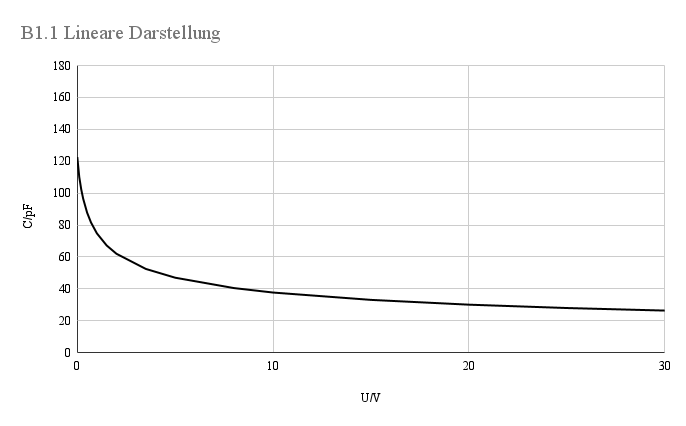
\includegraphics[width=0.7\textwidth]{B1.1LineareDarstellug}
	\caption{P600A Sperrschichtkapazität über Spannung.}
\end{figure}

%B1.2
\subsubsection{Sperrstrom}
Um den Vorwiderstand zu Dimensionieren wurde eine maximale Spannung von \SI{30}{\volt} gewählt sowie ein maximaler Strom von \SI{10}{\milli\ampere}.
\[
U = R \cdot I \quad \Leftrightarrow \quad I = \frac{U}{R}
\]
\[
R_{Vor} = \frac{\SI{30}{\volt}}{\SI{10}{\milli\ampere}} = \SI{3}{\kilo\ohm}
\]

Da es keinen exakten \SI{3}{\kilo\ohm} Widerstand gibt wurden \SI{5.1}{\kilo\ohm} gewählt.

Die Messung muss Stromrichtig erfolgen, da durch die Sperrpolung der Diode sehr kleine Ströme zu erwarten sind. Für hohe Spannungen ist es nicht essenziell die Spannung auf den Millivolt genau einzustellen. Auch bei \SI{0.5}{\volt} ist der erwartete Strom im Verhältnis zur Spannung sehr gering. 
Das Picoampermeter wird am niederohmigen Knoten geschaltet, um den sehr kleinen Sperrstrom möglichst genau messen zu können. Dabei ist zu beachten, dass der Spannungsabfall über das Messgerät vernachlässigbar klein bleibt, damit die Messung nicht verfälscht wird.

\begin{table}[ht]
\centering
\begin{tabular}{c|cccccccccccccc}
U/\si{\volt} & 0,5 & 5 & 30\\
\hline
I/\si{\ampere} & 1,093\micro& 1,256\micro& 1,691\micro	\\
\end{tabular}
\caption{AA136 Sperrströme bei verschiedenen Spannungen.}
\label{tab:uv-cf}
\end{table}

\begin{table}[ht]
\centering
\begin{tabular}{c|cccccccccccccc}
U/\si{\volt} & 0,5 & 5 & 30\\
\hline
I/\si{\ampere} & 0,35\nano& 0,81\nano& 2,86\nano\\
\end{tabular}
\caption{1N4002 Sperrströme bei verschiedenen Spannungen.}
\label{tab:uv-cf}
\end{table}

\begin{center}
	Hinweis:  Der Sperrstrom bei 0,5V ist beim Messen zwsichen \SI{0.25}{\nano\ampere} und \SI{0.4}{\nano\ampere} geschwankt.
\end{center}


%B1.3
\subsubsection{Vorwärtsstrom 1N4002}

\begin{table}[H]
\centering
\begin{tabular}{c|cccccccc}
$U_R/\si{\volt}$ & 0 & 0.5 & 1 & 2 & 3 & 4 & 5 & 7.5 \\
$I/\si{\ampere}$ & 15 \nano& 30 \nano& 80 \nano& 150 \nano& 300 \nano& 800 \nano& 1.5 \micro& 3 \micro\\
\hline
$U_R/\si{\volt}$ & 10 & 12.5 & 15 & 20 & 25 & 30 & 2 & \\
$I/\si{\ampere}$ & 8\micro& 15\micro& 30\micro& 80\micro& 150\micro& 300\micro& 800\micro& \\
\end{tabular}
\caption{Sperrschichtstrom \(I/\si{\ampere}\) in Abhängigkeit von der Spannung \(U_R/\si{\volt}\).}
\label{tab:uv-cf}
\end{table}

\begin{figure}[H] % [H] forces the figure to be placed exactly where it appears in the text
	\centering % Horizontally center the figure
	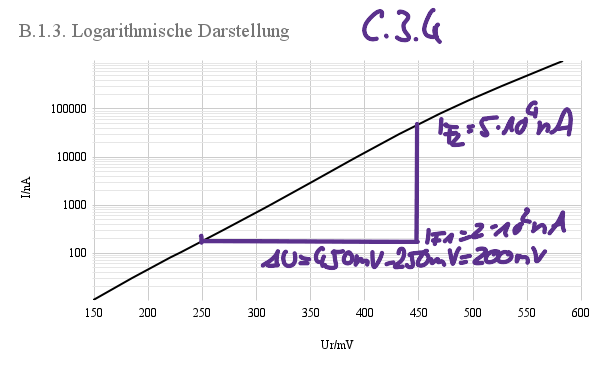
\includegraphics[width=0.7\textwidth]{B.1.3.LogarithmischeDarstellung} % Include the figure, now larger
	\caption{Logarithmische Darstellung des Durchlassstroms über Spannung der Diode 1N4002.}
\end{figure}


%B2
\subsection{Dynamische Aufnahme von Kennlinien}

%B2.1
\subsubsection{Durchlaßkennlinien 1N4002 und AA136}
%Grafik Beginn
\begin{figure}[H] % [H] forces the figure to be placed exactly where it appears in the text
	\centering % Horizontally center the figure
	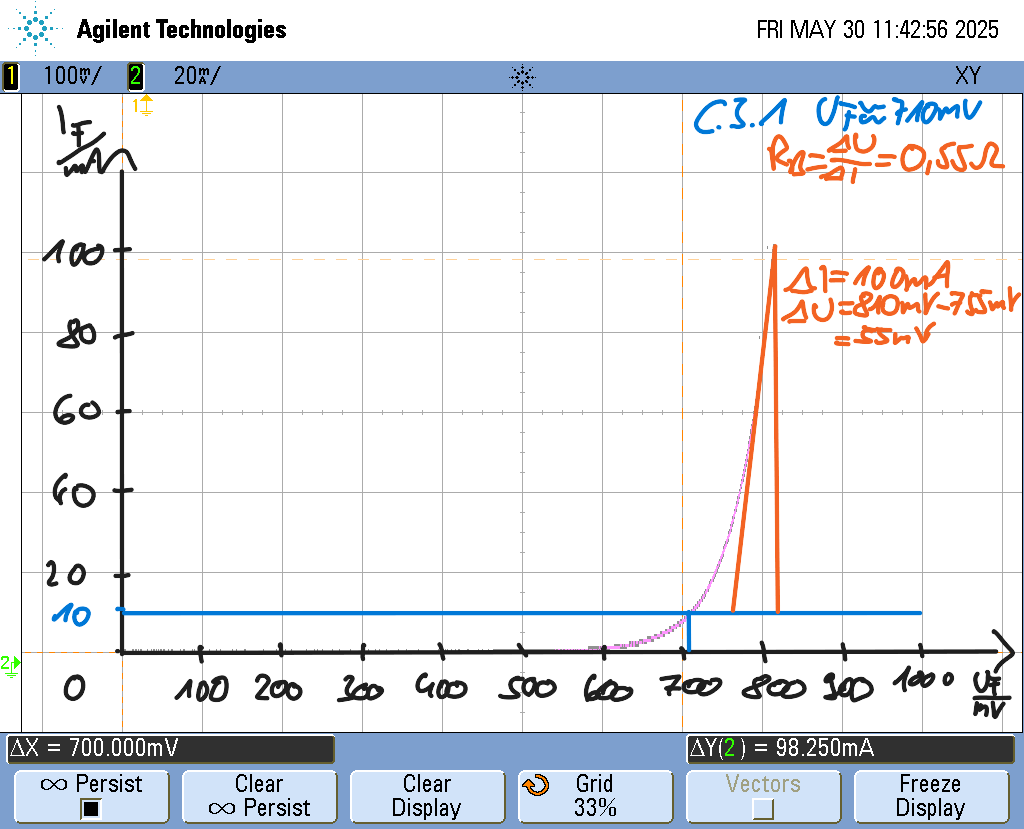
\includegraphics[width=0.75\textwidth]{B.2.1(1N4002)} % Include the figure, now larger
	\caption{1N4002 Durchlaßkennlinien. $R_B \approx \SI{0.55}{\ohm}$}
\end{figure}


%Grafik Ende
\begin{figure}[H] % [H] forces the figure to be placed exactly where it appears in the text
	\centering % Horizontally center the figure
	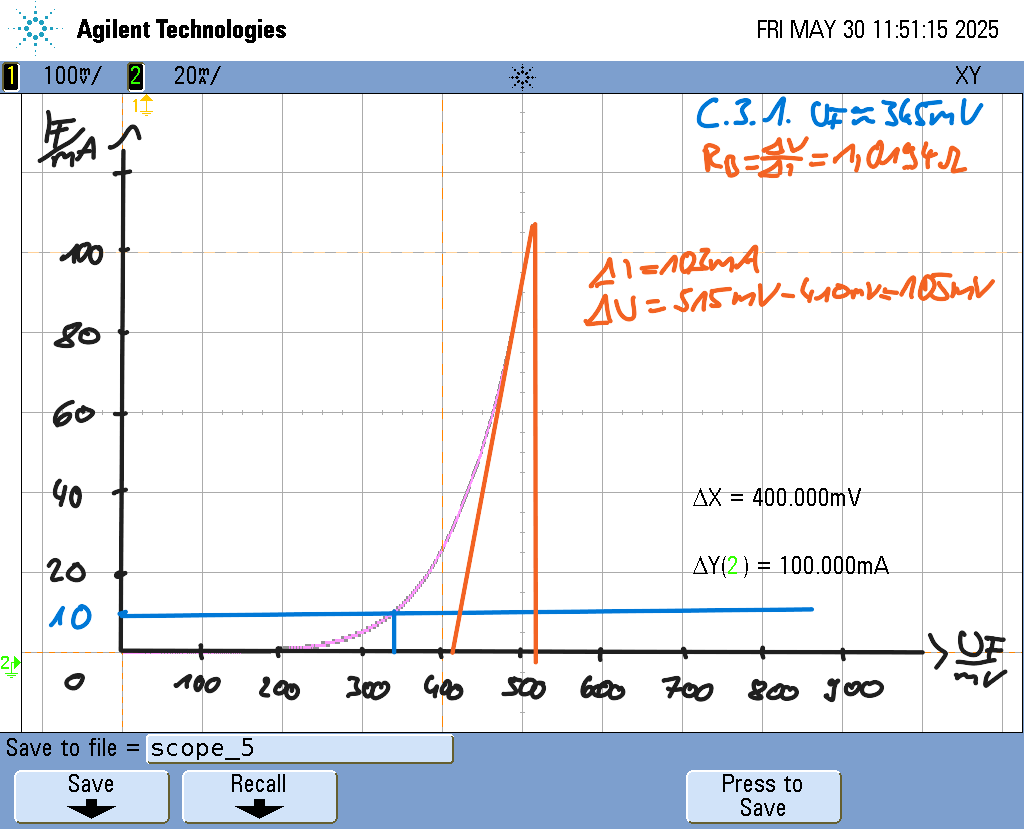
\includegraphics[width=0.75\textwidth]{B.2.1(AA136)} % Include the figure, now larger
	\caption{AA136 Durchlaßkennlinien}
\end{figure}


% \[
% I_F = \frac{U_Z}{0,1 \cdot 10}
% \]
% $I_{F}$ 
% $U_{Gen}= x$\ max.\ \SI{100}{\milli\ampere}


%B.2.2
\subsubsection{Vergleich der Kennlinien}
\begin{figure}[H] % [H] forces the figure to be placed exactly where it appears in the text
	\centering % Horizontally center the figure
	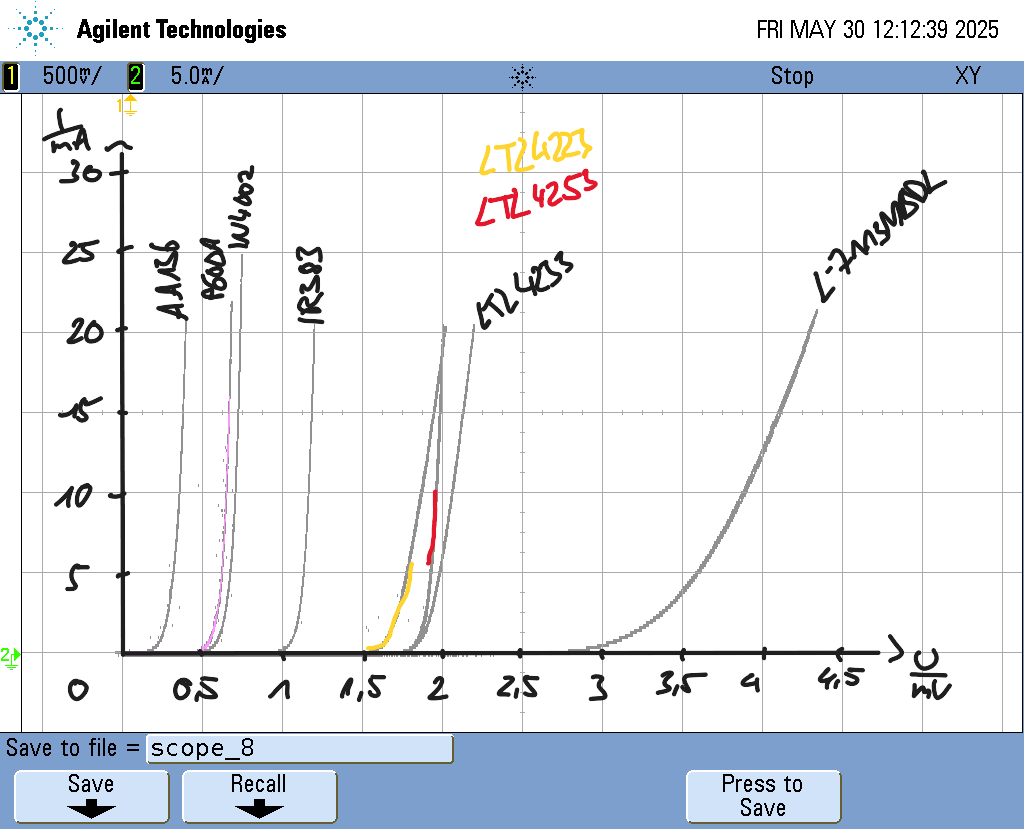
\includegraphics[width=0.75\textwidth]{B.2.2} % Include the figure, now larger
	\caption{Verschiedene Diodenkennlinien.}
\end{figure}

%B2.3.
\subsubsection{Z-Dioden}

\begin{figure}[H] % [H] forces the figure to be placed exactly where it appears in the text
	\centering % Horizontally center the figure
	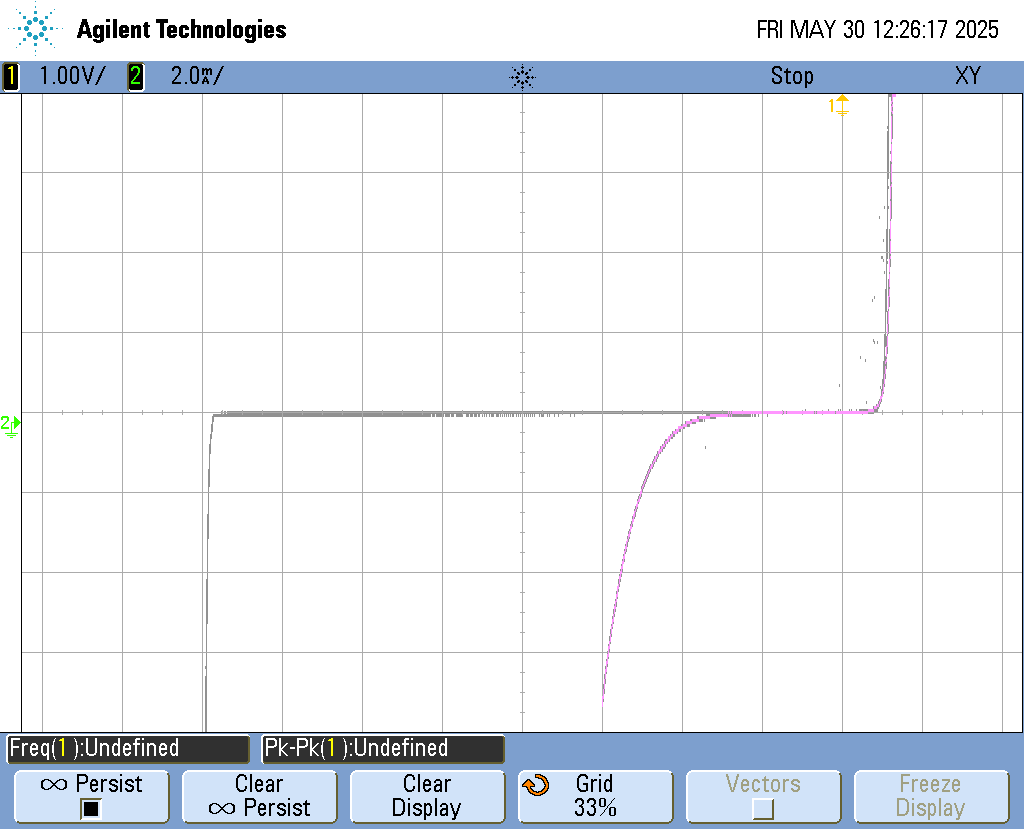
\includegraphics[width=0.75\textwidth]{B.2.3} % Include the figure, now larger
	\caption{Gesamtkennlinie der Zener Dioden ZPD8.2 und ZPD2.7.}
\end{figure}


%B.3
\subsection{Dynamisches Verhalten der Siliziumdiode (1N4002)}

%B.3.1
\subsubsection{Bestimmung von Speicher- und Abfallzeit}

\begin{figure}[H] % [H] forces the figure to be placed exactly where it appears in the text
	\centering % Horizontally center the figure
	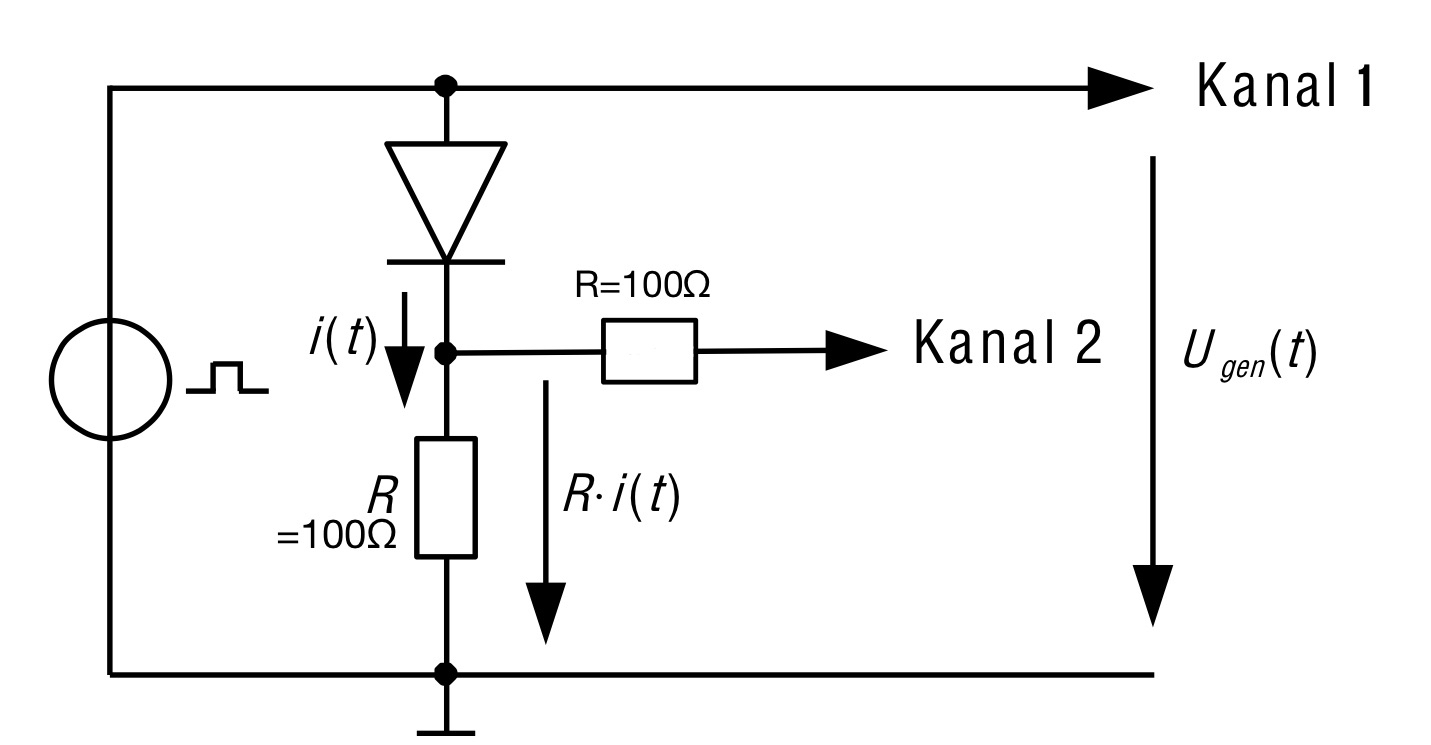
\includegraphics[width=0.6\textwidth]{B3.1a} % Include the figure, now larger
	\caption{Versuchsaufbau zur bestimmung der Speicher- und Abfallzeit.}
	\vspace{1em}
\end{figure}

\begin{figure}[H] % [H] forces the figure to be placed exactly where it appears in the text
	\centering % Horizontally center the figure
	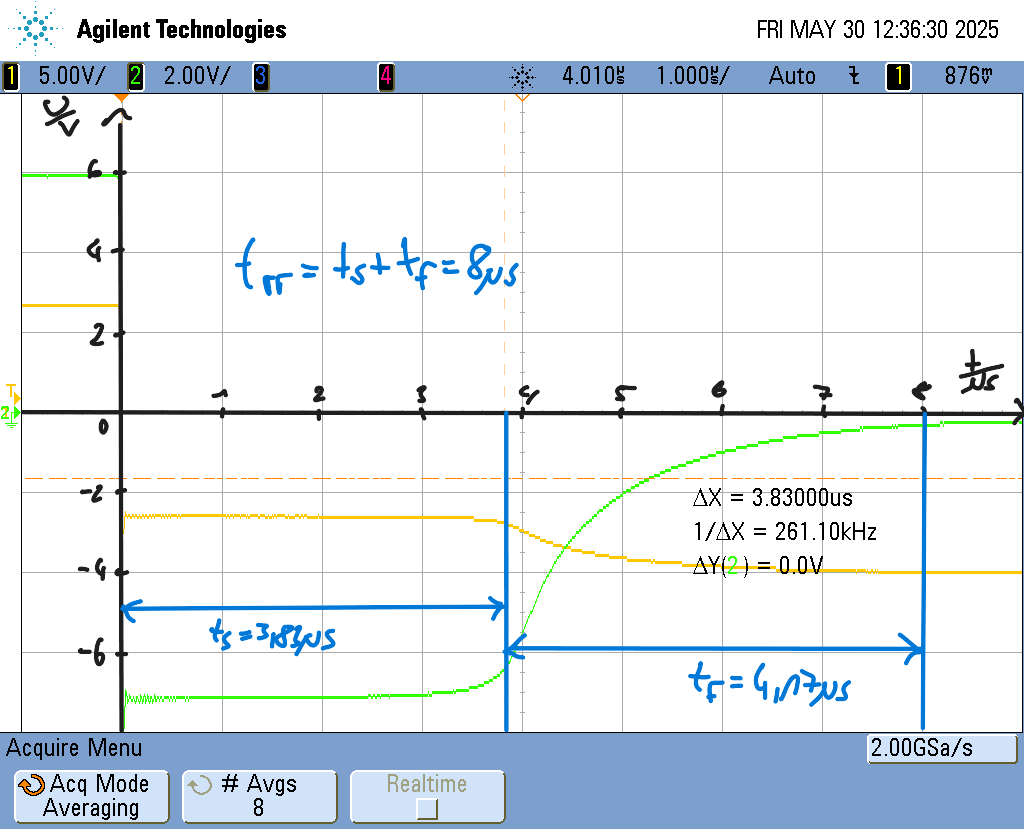
\includegraphics[width=0.75\textwidth]{B.3.1} % Include the figure, now larger
	\caption{Grafische bestimmung von $t_s$, $t_f$ und $t_{rr}$.}
\end{figure}

%B.3.2
\subsubsection{Bestimmung der Einschaltzeiten}
%$U_{pp} = 20V \quad f_{gen} = \SI{100}{\hertz}$\quad Funktion: Squarewave
\begin{figure}[H] % [H] forces the figure to be placed exactly where it appears in the text
	\centering % Horizontally center the figure
	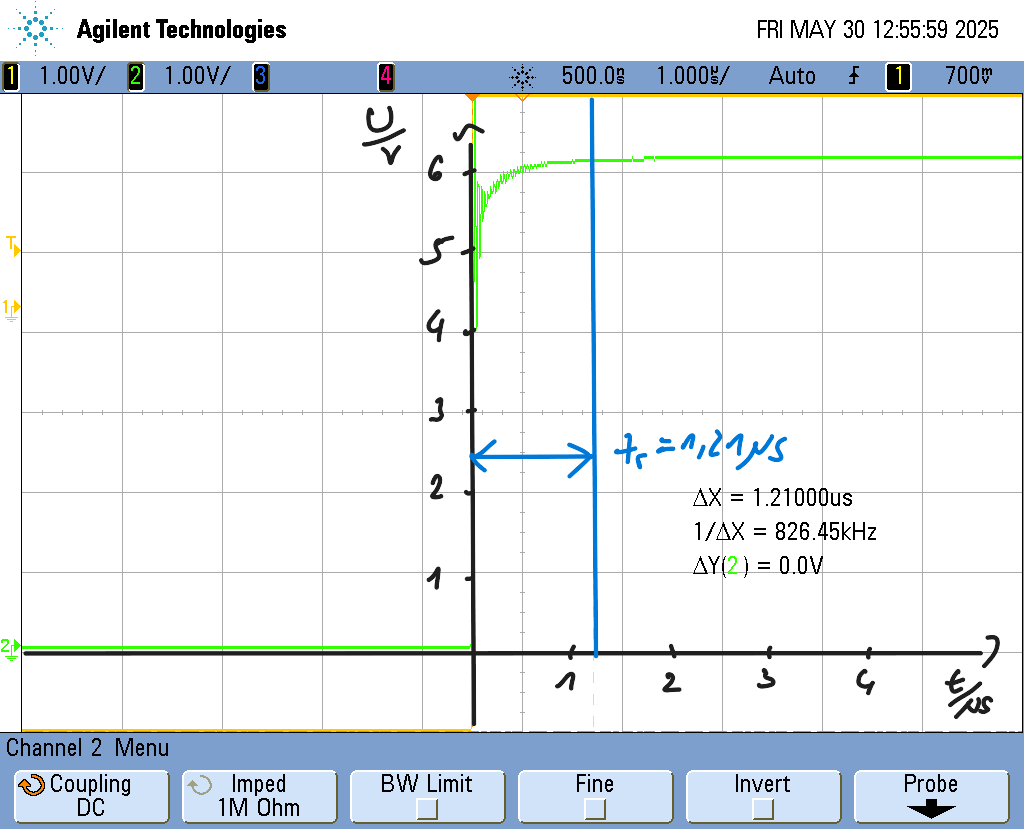
\includegraphics[width=0.75\textwidth]{B.3.2} % Include the figure, now larger
	\caption{Grafische bestimmung von $t_r$.}
	\vspace{1em}
\end{figure}

Nun soll die gesuchte Injektionszeit $t_i$ bestimmt werden. Erhöhen der Frequenz und beobachten der Speicherzeit ergab folgenden Wert für $f_{\text{best}}$: 

\begin{align*}
	f_{\text{best}} &= \SI{14,3}{\kilo\hertz} 
	&& t_r = \SI{1,21}{\micro\second}
\end{align*}

\begin{align*}
	\Rightarrow\quad 
    t_i &= \left(\frac{1}{2 f_{\text{best}}}\right) - t_r \\ \\
    t_i &= \SI{33,755}{\micro\second}
\end{align*}

%B.3.3
\subsubsection{Einfluß der Schaltzeiten auf die maximale Betriebsfrequenz}
\begin{figure}[H] % [H] forces the figure to be placed exactly where it appears in the text
	\centering % Horizontally center the figure
	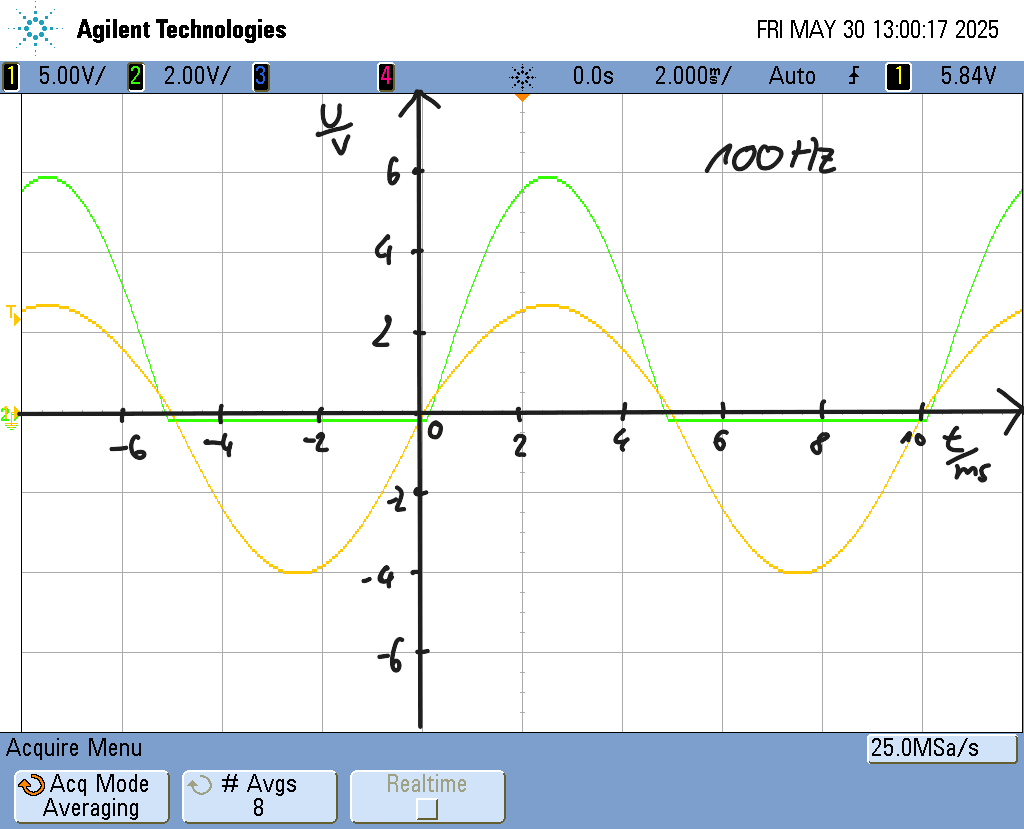
\includegraphics[width=0.75\textwidth]{B.3.3.a} % Include the figure, now larger
	\caption{Gleichrichtverhalten bei \SI{100}{\hertz}.}
\end{figure}
\begin{figure}[H] % [H] forces the figure to be placed exactly where it appears in the text
	\centering % Horizontally center the figure
	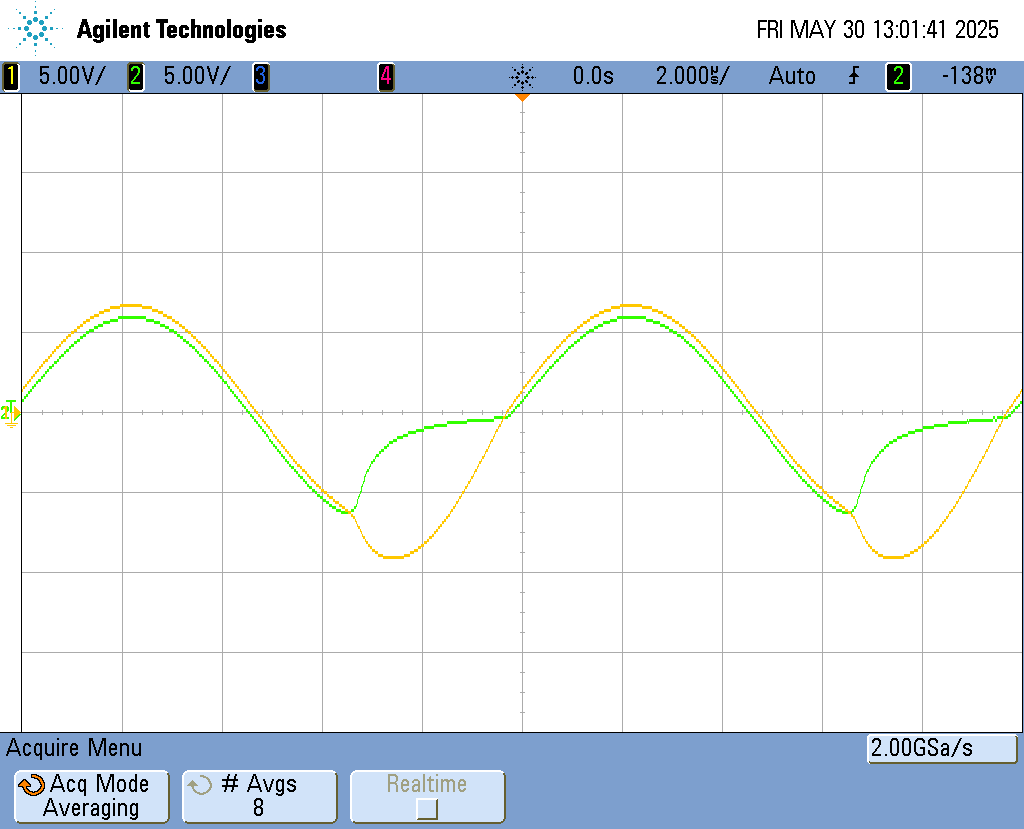
\includegraphics[width=0.75\textwidth]{B.3.3.b} % Include the figure, now larger
	\caption{Gleichrichtverhalten bei \SI{100}{\kilo\hertz}.}
\end{figure}
\begin{figure}[H] % [H] forces the figure to be placed exactly where it appears in the text
	\centering % Horizontally center the figure
	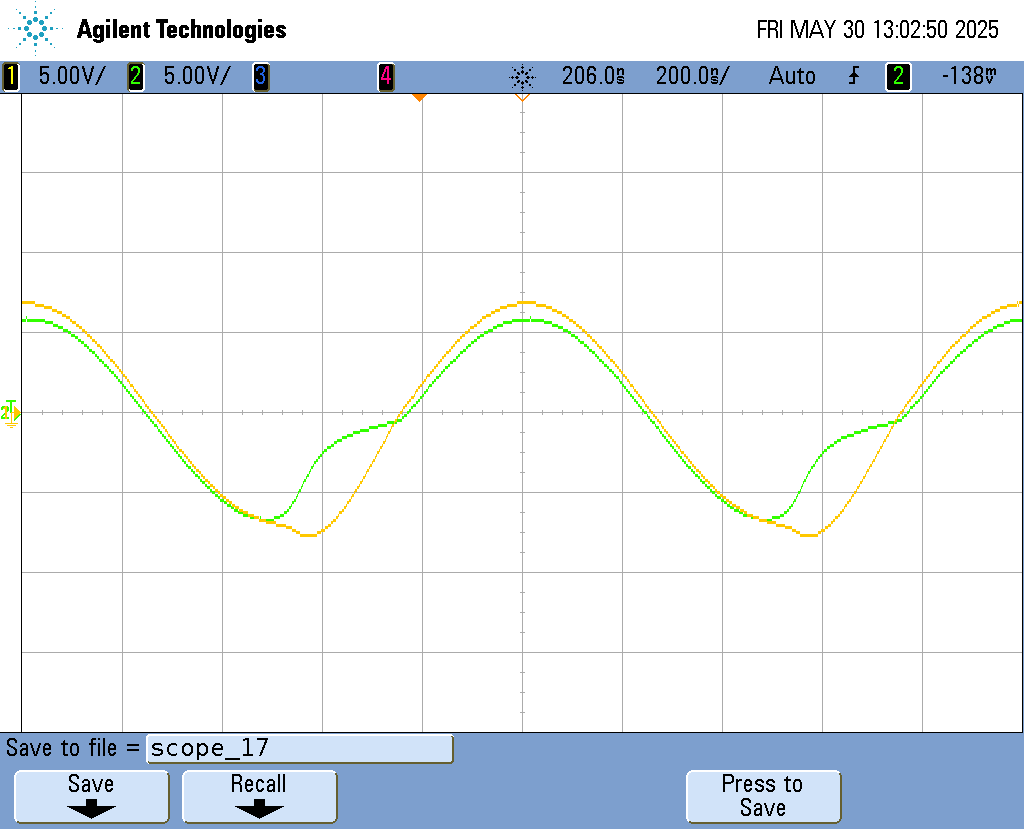
\includegraphics[width=0.75\textwidth]{B.3.3.c} % Include the figure, now larger
	\caption{Gleichrichtverhalten bei \SI{1}{\mega\hertz}.}
\end{figure}

\vspace{5em}

%B.3.4
\subsubsection{Dynamische Bestimmung des Bahnwiderstands}

\begin{figure}[H] % [H] forces the figure to be placed exactly where it appears in the text
	\centering % Horizontally center the figure
	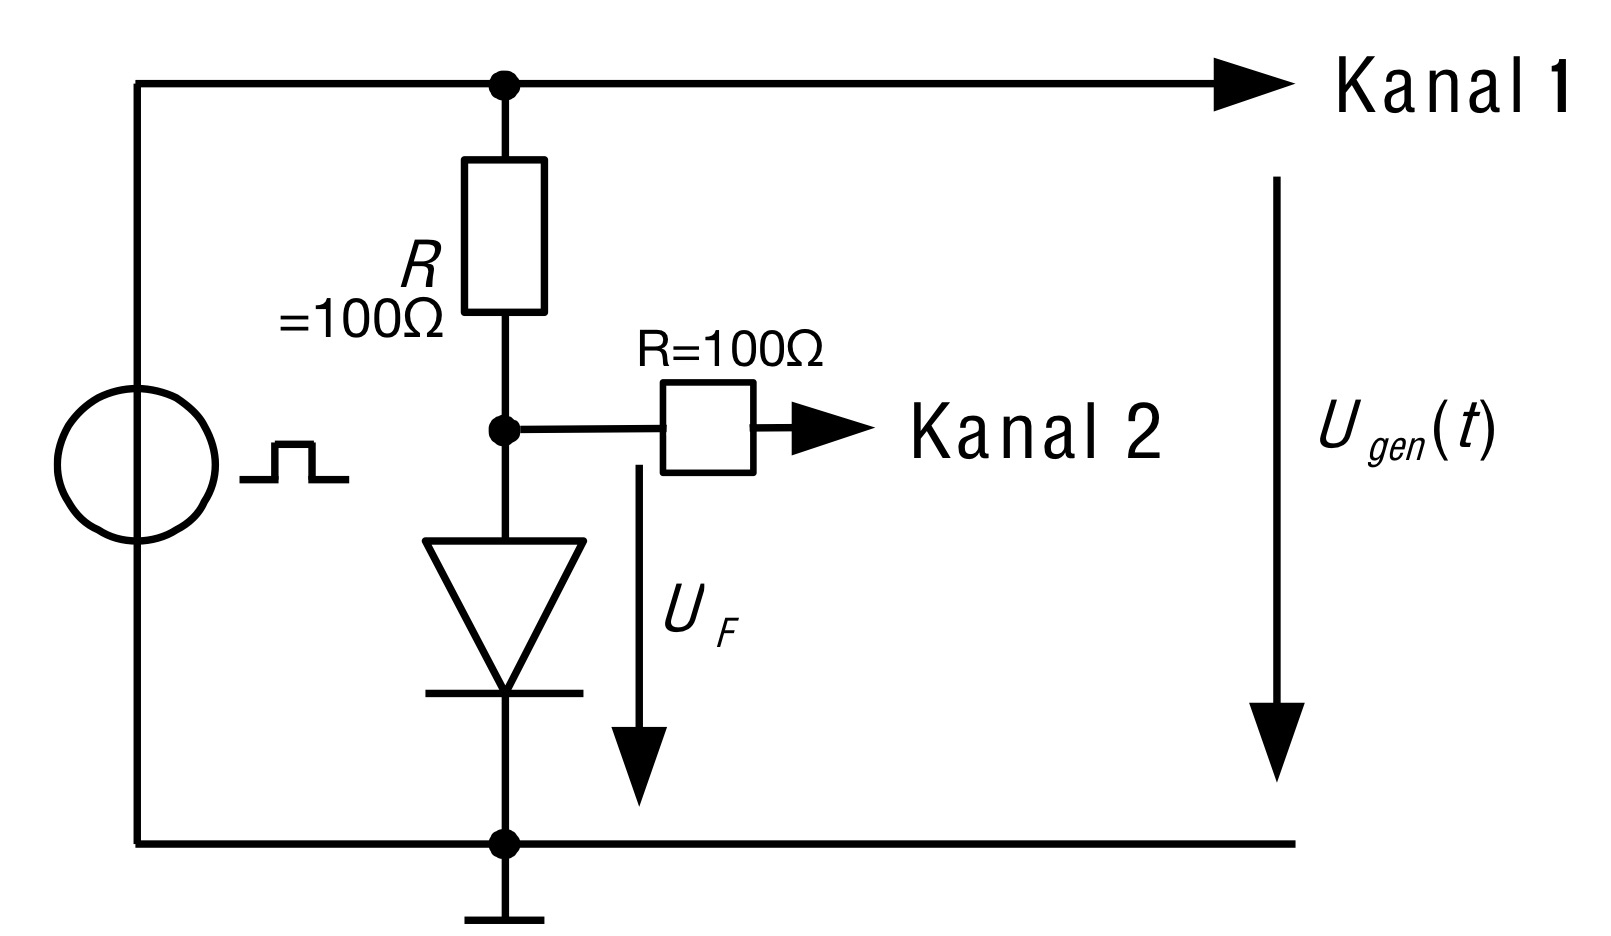
\includegraphics[width=0.6\textwidth]{B.3.4a} % Include the figure, now larger
	\caption{Versuchsaufbau zur Bestimmung des Bahnwiderstandes.}
\end{figure}

\begin{figure}[H] % [H] forces the figure to be placed exactly where it appears in the text
	\centering % Horizontally center the figure
	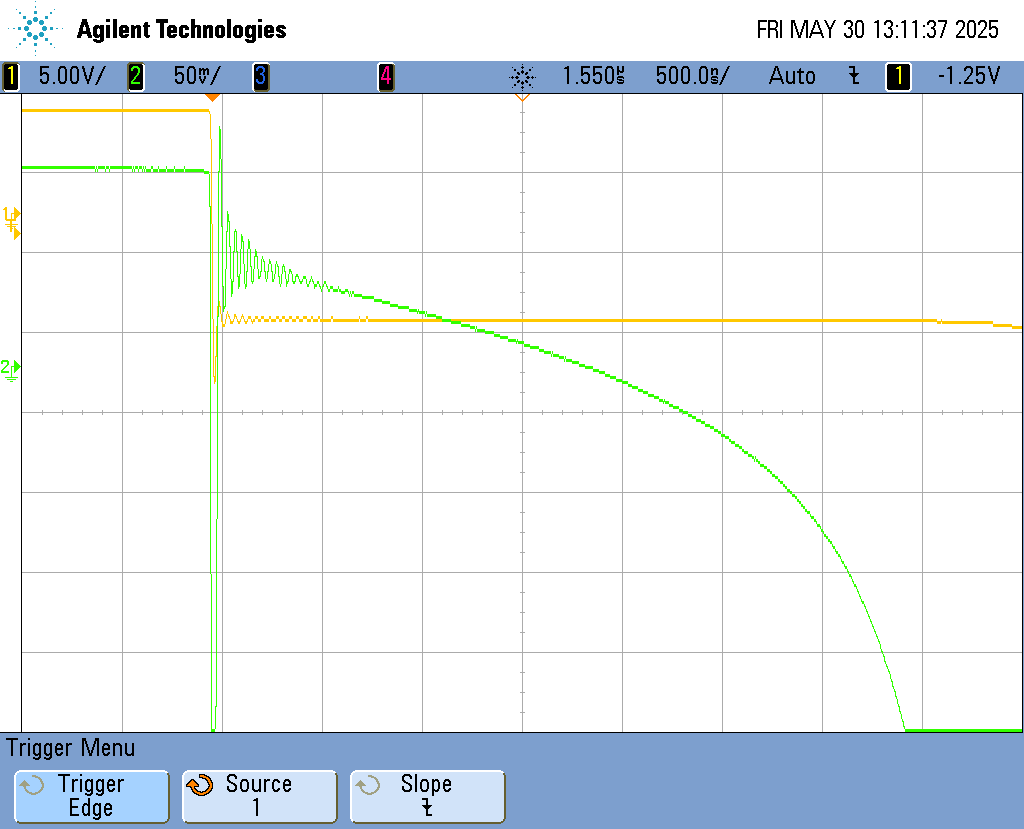
\includegraphics[width=0.75\textwidth]{B.3.4} % Include the figure, now larger
	\caption{Bestimmung des Spannungssprungs $U_D$.}
\end{figure}

\vspace{1em}

Anhand der gemessenen Werte kann nun $R_B$ bestimmt werden:

\begin{align*}
	\Delta U_{\text{gen}} &= \SI{13.5}{\volt} 
	&& \Delta U_D = \SI{50}{\milli\volt}
\end{align*}

\begin{align*}
	\Rightarrow\quad 
	R_B \approx \frac{\Delta U_D}{\Delta U_{\text{gen}} / R}
\end{align*}

\begin{align*}
	\Rightarrow\quad 
	R_B &= \frac{\SI{50}{\milli\volt}}{\SI{13.5}{\volt} / \SI{100}\ohm}  =  \SI{370}{\milli\ohm} \\
\end{align*}

\vspace{1em}


%C
\section{Auswertung}

%C.1
\subsection{Sperrschichtkapazität, Diffusionsspannung und \\Dotierstoffdichte}

\begin{figure}[H] % [H] forces the figure to be placed exactly where it appears in the text
	\centering % Horizontally center the figure
	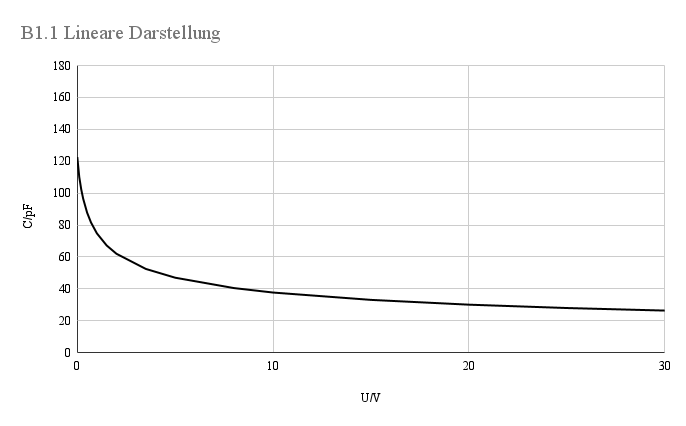
\includegraphics[width=0.75\textwidth]{B1.1LineareDarstellug} % Include the figure, now larger
	\caption{Sperrschichtkapazität über Spannung der P600A Diode.}
	\label{fig:Sperrschichtkap}
\end{figure}

\begin{figure}[H] % [H] forces the figure to be placed exactly where it appears in the text
	\centering % Horizontally center the figure
	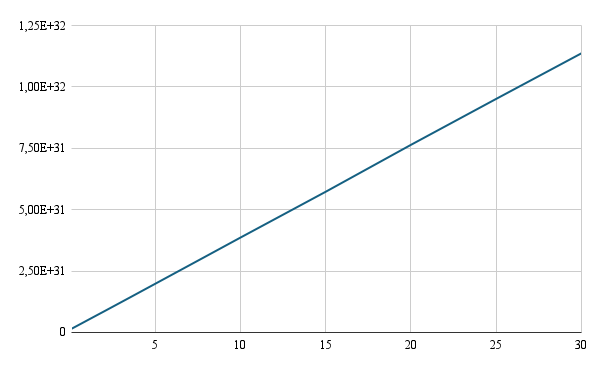
\includegraphics[width=0.75\textwidth]{C3.1faktore} % Include the figure, now larger
	\caption{$(\frac{1}{C})^2$ bei Stufenfaktor $M=0.33$.}
\end{figure}
\begin{figure}[H] % [H] forces the figure to be placed exactly where it appears in the text
	\centering % Horizontally center the figure
	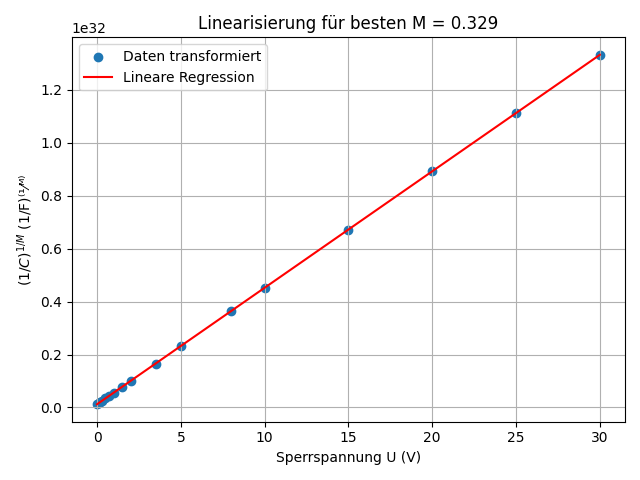
\includegraphics[width=0.75\textwidth]{mregression} % Include the figure, now larger
	\caption{Nichtlineare Regression in Python.}
\end{figure}

\[
C_S = \frac{C_{S0}}{(1+\frac{U}{U_D})^M}\quad f(U) = \frac{1}{C_S^\frac{1}{M}}
\]
Der Stufenfaktor wurde durch lineare Regression der Kapazitäts-Spannungs-Daten, abhänhih von M linearisiert. Die beste linearisierung entspricht in etwa dem Stufenfaktor. 
Der Schnittpunkt der Ausgleichsgerade mit der Spannungsachse entspricht der Diffusionsspannung $U_D$ (hier $\approx \SI{0.275}{\volt}$).
Stufenfaktor von $M \approx 3.33$ ist ein indiz für einen abrupten pn-Übergang. \\
Das hierbei verwendete Python Skript findet sich im Anhang.


% TODO: Replace 0 with the actual value 

\[
U_D = \SI{0.275}{\volt} \quad C_{S0} = \SI{122,6}{\pico\farad} \quad \varepsilon_{\mathrm{r,Si}} = 11{,}7 \quad A_{RLZ} = \SI{2.5}{\milli\metre\squared}
\]

\begin{align*}
N_A &\gg N_D \rightarrow \text{abrupter pn-Übergang} \\
\rightarrow\ C_{s0} &= \sqrt{\frac{\varepsilon_r \cdot \varepsilon_0 \cdot e N_D \cdot N_A}{2 \cdot (N_D + N_A) \cdot U_D}} \cdot A_{RLZ} \\
\leftrightarrow\ N_D &= \frac{C_s^2 \cdot 2 \cdot (U_D - U)}{\varepsilon_r \cdot \varepsilon_0 \cdot A_{RLZ}^2}
\end{align*}
\[
N_D \approx \SI{84.04e12}{\per\centi\meter\cubed}
\]
\vspace{1em} 
\[
	U_{db} \approx \SI{10}{\volt}(10^{17} \cdot N_D^{-1}) \rightarrow U_{db} > 1400 \text{also plausibel}
\]
%C.2
\subsection{Vergleich verschiedener Dioden}
Für Vergleich in Übersichtsdarstellung siehe B.2.2 Grafik.
\[
\left.
\begin{array}{l}
W_g = h \cdot f \\
\lambda = \frac{c}{f}
\end{array}
\right\}
\quad \lambda = \frac{c\cdot h}{W_g} \cdot e \leftrightarrow W_g = \frac{c \cdot h}{\lambda \cdot e}
\]
Daraus folgt $\lambda = x$. \\

\[
\left.
\begin{array}{l}
I|_{U>3U_T} = I_S\cdot e^{U/U_T} \leftrightarrow U = U_T\cdot ln(\frac{I}{I_S}) \\
I_{S_{lang}} = q A n_i^2 \left( \frac{D_p}{L_p N_D} + \frac{D_n}{L_n N_A} \right) \\
n_i^2 = \sqrt{N_C N_V} \cdot \exp\left(-\frac{W_g}{2kT}\right)
\end{array}
\right\}
\quad I_s \varpropto n_i^2 \varpropto \exp\left(-\frac{W_g}{2kT}\right)
\]

\vspace{1em} 

Desto kleiner $I_s$ bzw. desto größer $W_g$, umso größer muss $U$ sein, um einen Strom $I$ zu halten.\\  
Dies führt zu einer größeren bzw. kleineren Bandlücke:\\

% Bandlücken aller Dioden aus Abbildung 4.\\
% AA136 (Germanium) \( W_g = 0{,}67\,\text{eV} \)\\
% P600A, IN4002 (Silizium) \( W_g = 1{,}12\,\text{eV} \)\\
% IR383 (\( \lambda = 940\,\text{nm} \)) \( W_g = 1{,}32\,\text{eV} \)\\
% LTL-4253 (\( \lambda = 585\,\text{nm} \)) \( W_g = 2{,}12\,\text{eV} \)\\
% LTL-4223 (\( \lambda = 635\,\text{nm} \) \( W_g = 1{,}95\,\text{eV} \)\\
% LTL-4233 (\( \lambda = 565\,\text{nm} \)) \( W_g = 2{,}19\,\text{eV} \)\\
% L-7113MBDL (\( \lambda = 430\,\text{nm} \)) \( W_g = 2{,}88\,\text{eV} \)

\begin{table}[h]
\centering
\begin{tabular}{lll}
\toprule
\textbf{Diode} & \textbf{Wellenlänge \(\lambda\)} & \textbf{Bandlücke \(W_g\) [eV]} \\
\midrule
AA136 (Germanium)     & --              & 0{,}67 \\
P600A (Silizium)      & --              & 1{,}12 \\
1N4002 (Silizium)     & --              & 1{,}12 \\
IR383 (IR-LED)        & 940\,nm         & 1{,}32 \\
LTL-4253 (Gelb-LED)   & 585\,nm         & 2{,}12 \\
LTL-4223 (Rot-LED)    & 635\,nm         & 1{,}95 \\
LTL-4233 (Grün-LED)   & 565\,nm         & 2{,}19 \\
L-7113MBDL (Blau-LED) & 430\,nm         & 2{,}88 \\
\bottomrule
\end{tabular}
\caption{Bandlücken der verschiedenen Dioden}
\end{table}


%C.3
\subsection{Schaltdioden}

%C.3.1
\subsubsection{Kennlinienparameter}
Für graphische Darstellung für $U_F$ und $R_B$ siehe B.2.1. \\
$U_{Z_{\SI{5}{\milli\ampere}}}$ wird bei B.2.3 grafisch Bestimmt. \\

\begin{table}[H]
\centering
\begin{tabular}{l|llll}
							& $U_{\text{F,Datenblatt}}$ & $U_{F,\text{Gemessen}}$ & $R_{B,\text{Datenblatt}}$ & $R_{B,\text{Gemessen}}$ \\
\hline
1N4002                     & \SI{0.93}{\volt}                        & \SI{0.71}{\volt}                       & N.A                          & \SI{0.55}{\ohm}                         \\
\hline
AA136                      & \SI{0.55}{\volt}                        & \SI{0.345}{\volt}                      & N.A                          & \SI{1.0194}{\ohm}                       \\                       
\end{tabular}
\end{table}

Da im Datenblatt nur sehr schwammige Aussagen über die Forward-Spannung getroffen werden und keine Aussage über den Bahnwiderstand ist es schwierig die werte zu vergleichen.



\begin{figure}[H] % [H] forces the figure to be placed exactly where it appears in the text
	\centering % Horizontally center the figure
	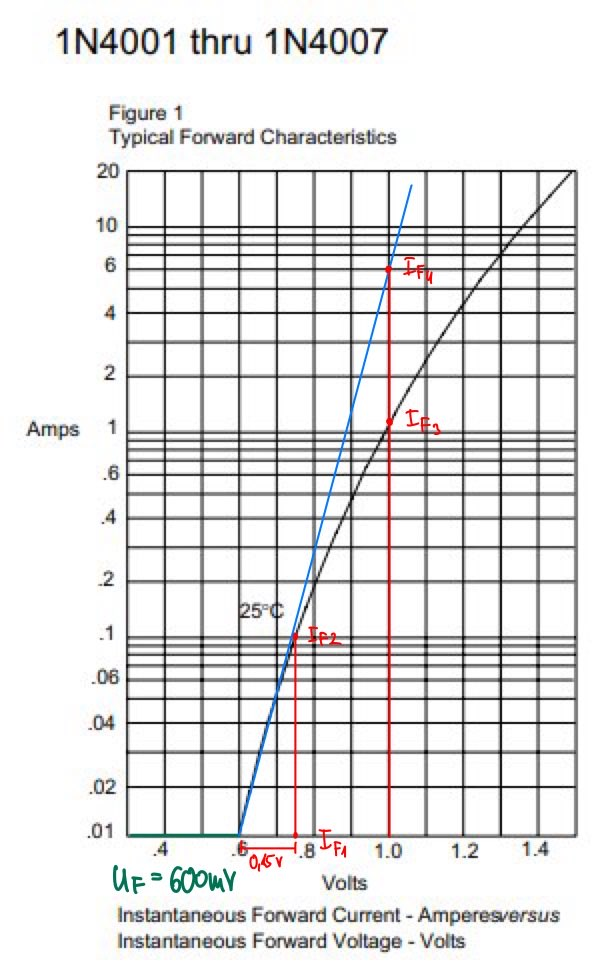
\includegraphics[width=0.6\textwidth]{C.3.1c 1N4002} % Include the figure, now larger
	\caption{Grafische bestimmung von $U_F$ und $R_B$.}
\end{figure}

\begin{figure}[H] % [H] forces the figure to be placed exactly where it appears in the text
	\centering % Horizontally center the figure
	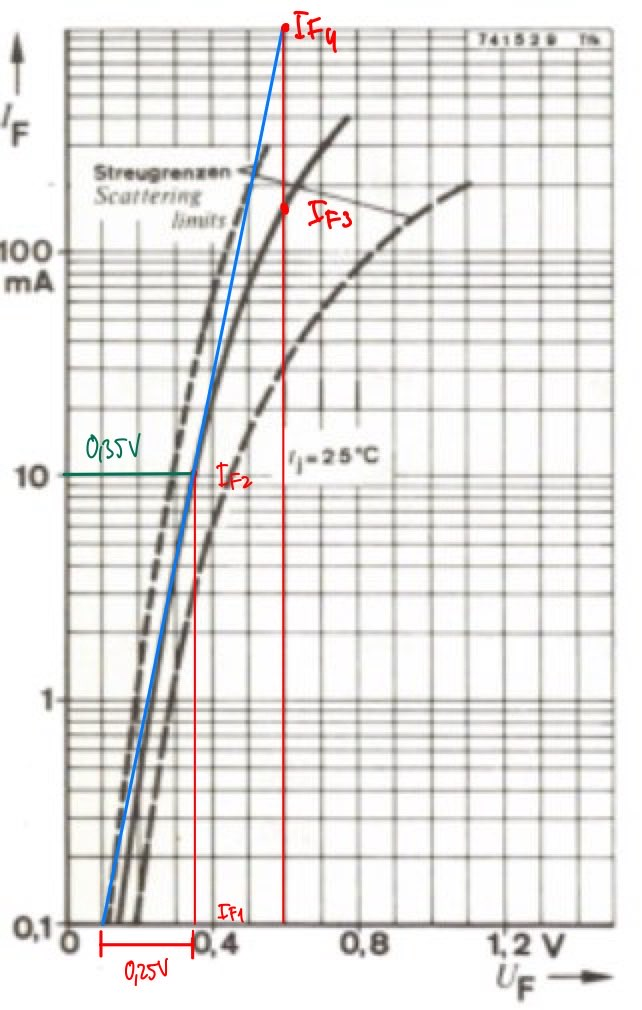
\includegraphics[width=0.6\textwidth]{C.3.1c2 1N4002} % Include the figure, now larger
	\caption{AA136 Grafische Bestimmung von $U_F$ und $R_B$.}
\end{figure}

\vspace{2em}

Die Berechnung der Bahnwiderstände ergibt:\\

a) 1N4002:

\begin{equation*}
\begin{array}{c@{\hspace{3cm}}c}
m = \frac{\Delta U_F}{U_T \cdot \ln\left( \frac{I_{F2}}{I_{F1}} \right)} = 0{,}02525
& R_B = \frac{m \cdot U_T}{I_{F1}} \cdot \ln\left(\frac{I_{F0}}{I_{F1}}\right) = \SI{87,572}{\milli\ohm}
\end{array}
\end{equation*}

b) AA136:

\begin{equation*}
\begin{array}{c@{\hspace{3cm}}c}
m = \frac{\Delta U_F}{U_T \cdot \ln\left( \frac{I_{F2}}{I_{F1}} \right)} = 4{,}2083
& R_B = \frac{m \cdot U_T}{I_{F1}} \cdot \ln\left(\frac{I_{F0}}{I_{F1}}\right) = \SI{1,172}{\ohm}
\end{array}
\end{equation*}

\begin{figure}[H] % [H] forces the figure to be placed exactly where it appears in the text
	\centering % Horizontally center the figure
	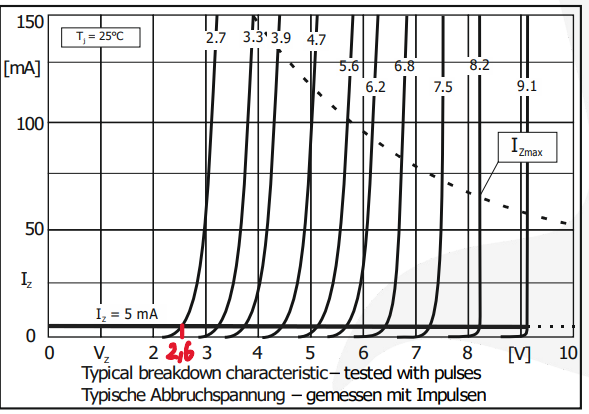
\includegraphics[width=0.6\textwidth]{C.3.1 Z2.7 zenerdiode} % Include the figure, now larger
	\caption{Grafische Bestimmung der Zenerspannung von ZPD2.7.}
\end{figure}

\vspace{3em}

\begin{figure}[H] % [H] forces the figure to be placed exactly where it appears in the text
	\centering % Horizontally center the figure
	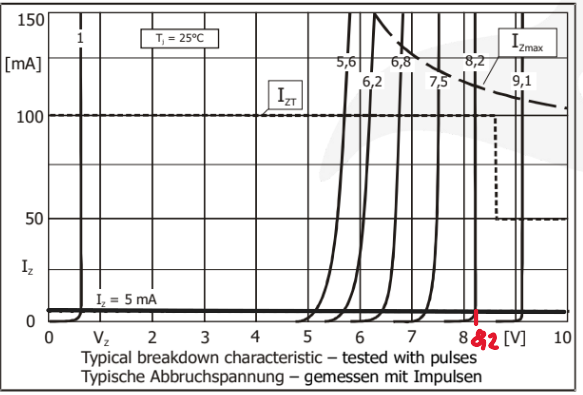
\includegraphics[width=0.6\textwidth]{C.3.1 Z8.2 zenerdiode} % Include the figure, now larger
	\caption{Grafische bestimmung der Zenerspannung von ZPD8.2.}
\end{figure}

\begin{table}[H]
\centering
\begin{tabular}{l|ll}
                            & $U_{\text{Z,Datenblatt}}$ & $U_{Z,\text{Gemessen}}$ \\
\hline
ZPD2.7                      &\SI{2,6}{\volt}                        &\SI{2,8}{\volt}                      \\
\hline
ZPD8.2                      &\SI{8,2}{\volt}                        &\SI{7,95}{\volt}                      \\                       
\end{tabular}
\end{table}

Die gemessenen Werte stimmen im Rahmen der Messgenauigkeit mit den Werten aus dem Datenblatt überein.

%C.3.2
\subsubsection{Bahnwiderstand}
$R_{B1N4002\text{B3.4}} = \SI{370}{\milli\ohm}$ \qquad\qquad $R_{B1N4002\text{C3.1}} = \SI{87.572}{\milli\ohm}$\\\\
%----------------------------------------------------------------------------------------
%	SAMPLE CALCULATION
%----------------------------------------------------------------------------------------

%C.3.3
\subsubsection{Ideale Kennlinie}
Für zeichnerisch dargstellte Idealkennlinie siehe B.2.1.

%C.3.4

\subsubsection{Sperrsättigungsstrom und Emissionskoeffizient 1N4002}
\begin{figure}[H] % [H] forces the figure to be placed exactly where it appears in the text
	\centering % Horizontally center the figure
	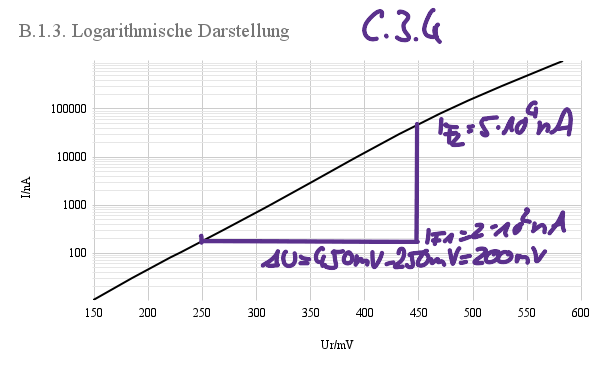
\includegraphics[width=0.6\textwidth]{B.1.3.LogarithmischeDarstellung} % Include the figure, now larger
	\caption{$\Delta U$, $I_{F1}$ und $I_{F2}$}
\end{figure}
\begin{figure}[H] % [H] forces the figure to be placed exactly where it appears in the text
	\centering % Horizontally center the figure
	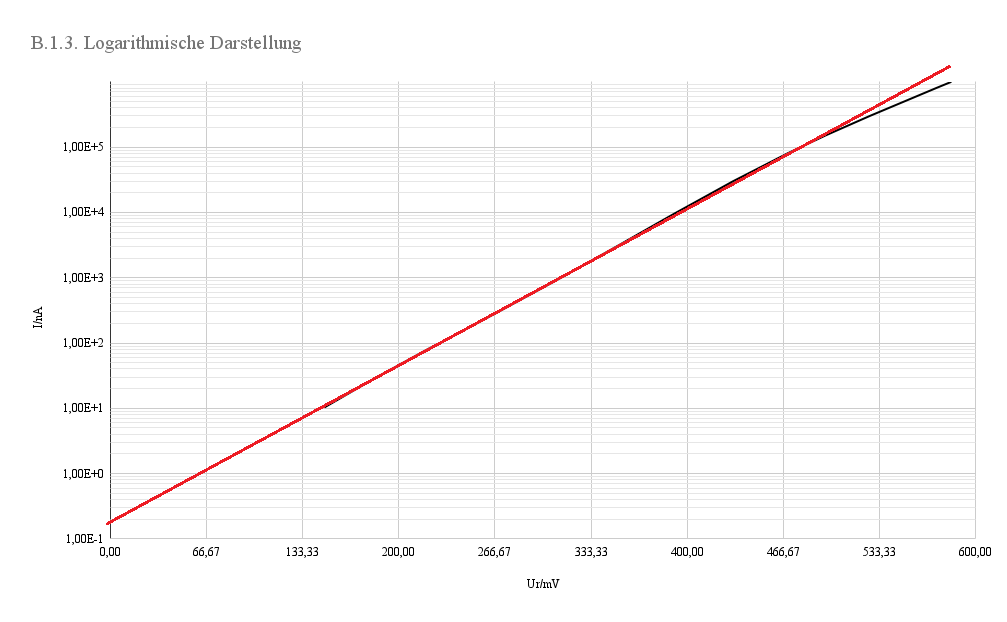
\includegraphics[width=0.6\textwidth]{Geradelog} % Include the figure, now larger
	\caption{Grafische Bestimmung von $I_S$ bei $\approx \SI{0.2}{\nano\ampere}$}
\end{figure}
\vspace{1em} 
\[
\Delta U_F = \SI{200}{\milli\volt} \quad \frac{I_{F2}}{I_{F1}} = 2.5\cdot10^2
\]
\[
m = \frac{\Delta U_F}{\SI{25.8}{\milli\electronvolt}\cdot \ln(I_{F2}/I_{F1})} \rightarrow m \approx 1,4
\]
\vspace{1em}

Verlauf Durchlaßkennlinien siehe B2.1.\\

Zudem sind Temperaturabhängigkeiten sowie Messgenauigkeiten und Verunreinigungen mögliche Ursachen. 

$I_{S Grafisch} = \SI{0.2}{\nano\ampere} < I_{S B1.2}$. Diese Abweichung lässt sich auf thermischer Generation zurückzuführen. Für größere $U_R$ weitet sich die RLZ aus, wodurch thermische Generation einen größeren Einfluss hat. 
\[
I_F = I_S(e^{U/\SI{25.8}{\milli\electronvolt}}-1)
\]

In der gemessenen Kennlinie werden reale Parameter wie Leitungswiderstamd, nichtideales Verhalten des Halbleiters sowie Temperaturabhängigkeiten abgebildet.
Der Emissionskoeffizient passt dabei die Idealkennlinie etwas an die gemessene an. Trotzdem besteht noch eine nähere Übereinstimmung mit der idealen Kennlinie.

%C.3.5
\subsubsection{Schaltverhalten}

\vspace{1em} 

\begin{center}
\begin{tabular}{ll}
\toprule
\textbf{Symbol} & \textbf{Wert} \\
\midrule
Anstiegszeit      & $\SI{1.21}{\micro\second}$ \\
Einschaltzeit     & $\SI{33.755}{\micro\second}$ \\
Speicherzeit      & $\SI{3.83}{\micro\second}$\\
Abfallzeit        & $\SI{4.17}{\micro\second}$  \\
Rückerholzeit     & $\SI{8}{\micro\second}$ \\
\bottomrule
\end{tabular}
\end{center}

\vspace{1em} 

Zu erwarten wäre eine Funktion ähnlich $y = \hat{u}\sin(x) \text{ für } y < 0 \rightarrow 0$.\par
Bei hohen Frequenzen können Dioden den Strom nicht mehr ideal gleichrichten, da ihre Schaltzeiten begrenzt sind. Besonders durch die Speicherzeit fließt nach dem Umschalten kurzzeitig ein Rückstrom. Auch die Rückerholzeit führt zu negativen Stromimpulsen beim Sperren. Dadurch entstehen bei höheren Frequenzen Verzerrungen im Stromverlauf, da die Diode nicht mehr rechtzeitig schalten kann.

%----------------------------------------------------------------------------------------
%	BIBLIOGRAPHY
%----------------------------------------------------------------------------------------

%\section{Formelzeichen}
\begin{table}[h]
\centering
\begin{tabular}{ll}
\toprule
\textbf{Symbol} & \textbf{Bedeutung} \\
\midrule
$C_s$    & Sperrschichtkapazität \\
$I_c$    & Fluß- oder Vorwärtestrom \\
$I_a$    & Sperrstrom- oder Rückwärtestrom \\
$I_s$    & Sperrsättigungsstrom \\
$M$      & Stufenfaktor (grading coefficient) \\
$m$      & Emissionskoeffizient \\
$N_a$    & Akzeptordichte \\
$N_0$    & Donatordichte \\
$R_a$    & Bahnwiderstand \\
$t_0$    & Injektionszeit \\
$t_1$    & Anstiegszeit (Risetime) \\
$t_1$    & Sperrverzögerungszeit (Reverse Recovery Time) \\
$t_s$    & Speicherzeit \\
$U_0$    & Diffusionsspannung \\
$U_c$    & Fluß- oder Vorwärtsspannung \\
$U_s$    & Sperr- oder Rückwärtsspannung \\
$U_{s\_5mk}$ & Durchbruchspannung an der Z-Diode bei $I_2 = 5$mA \\
\bottomrule
\end{tabular}
\end{table}


\printbibliography % Output the bibliography
\clearpage
%----------------------------------------------------------------------------------------
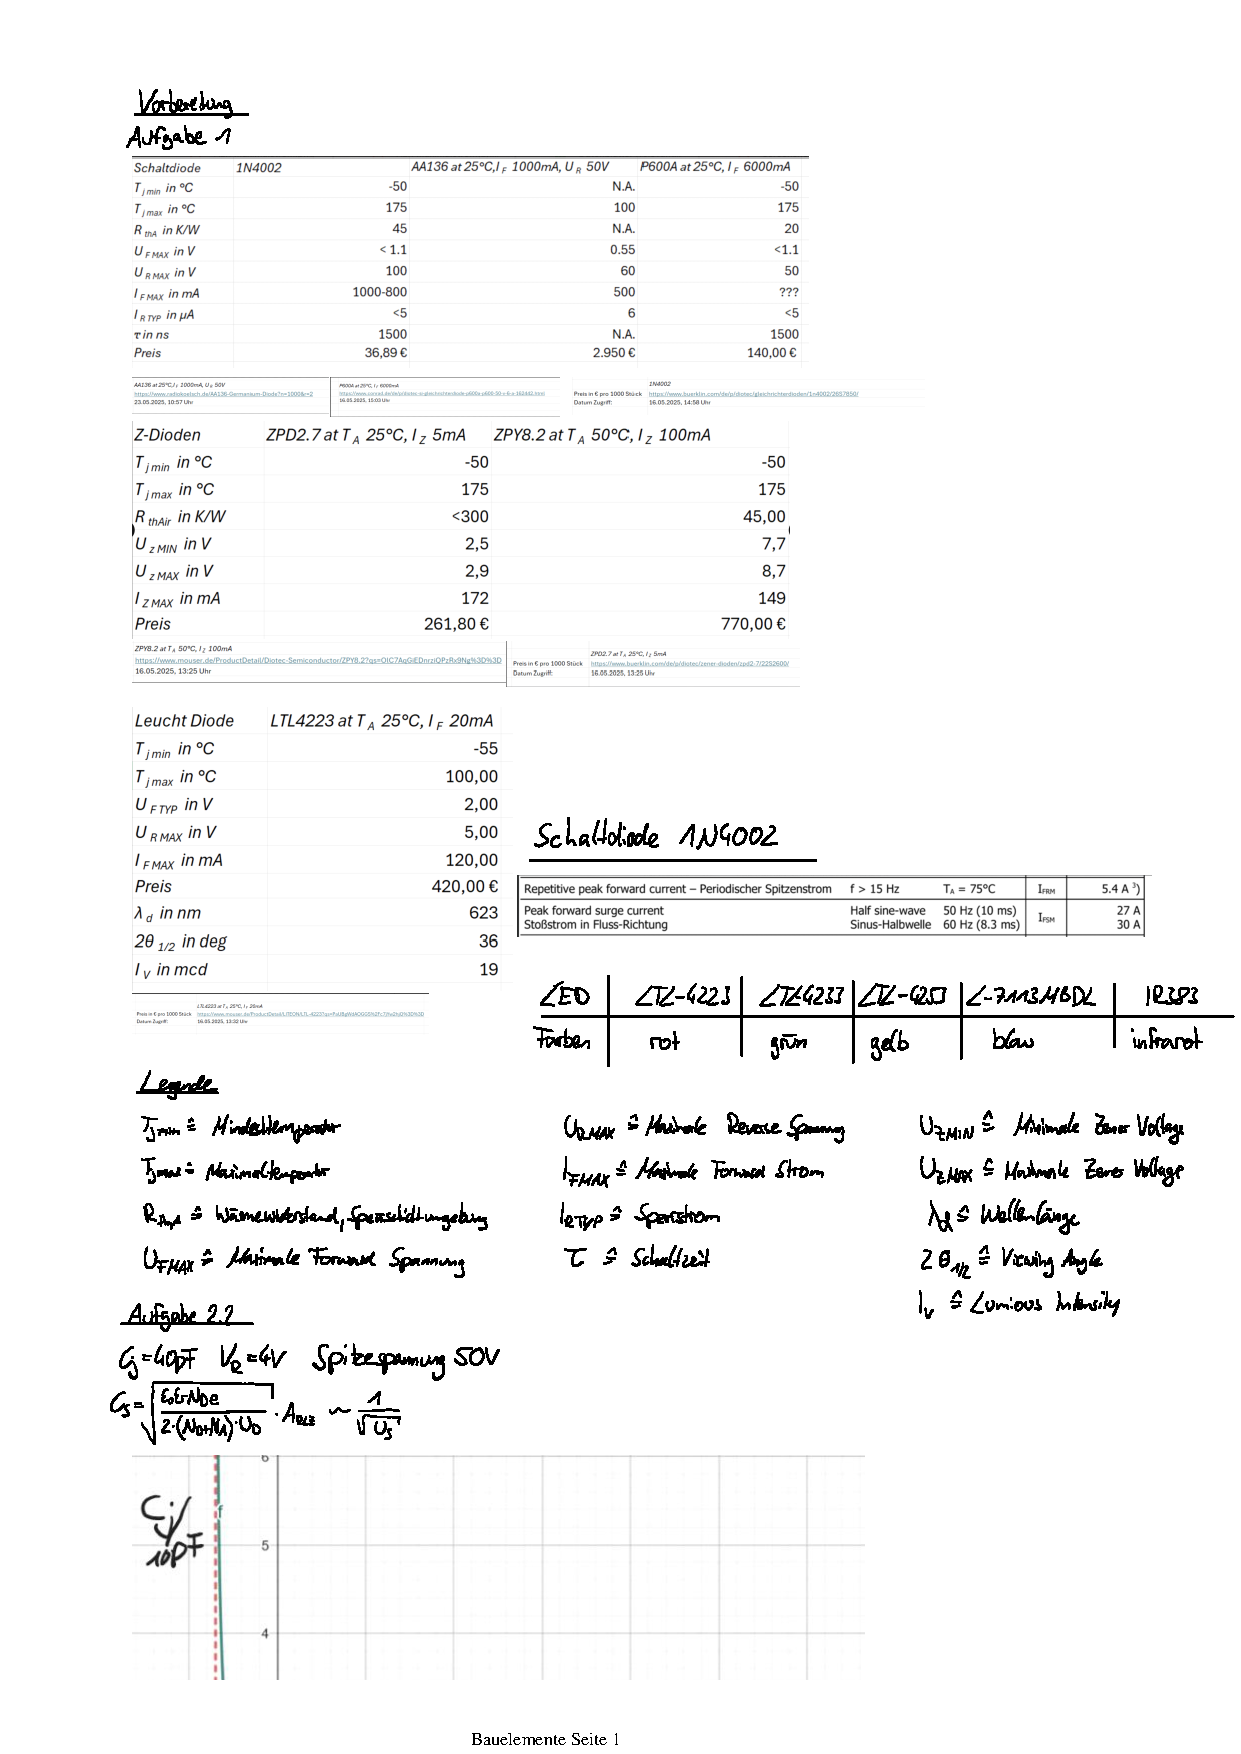
\includepdf[pages=-]{Vorbereitung1.pdf}
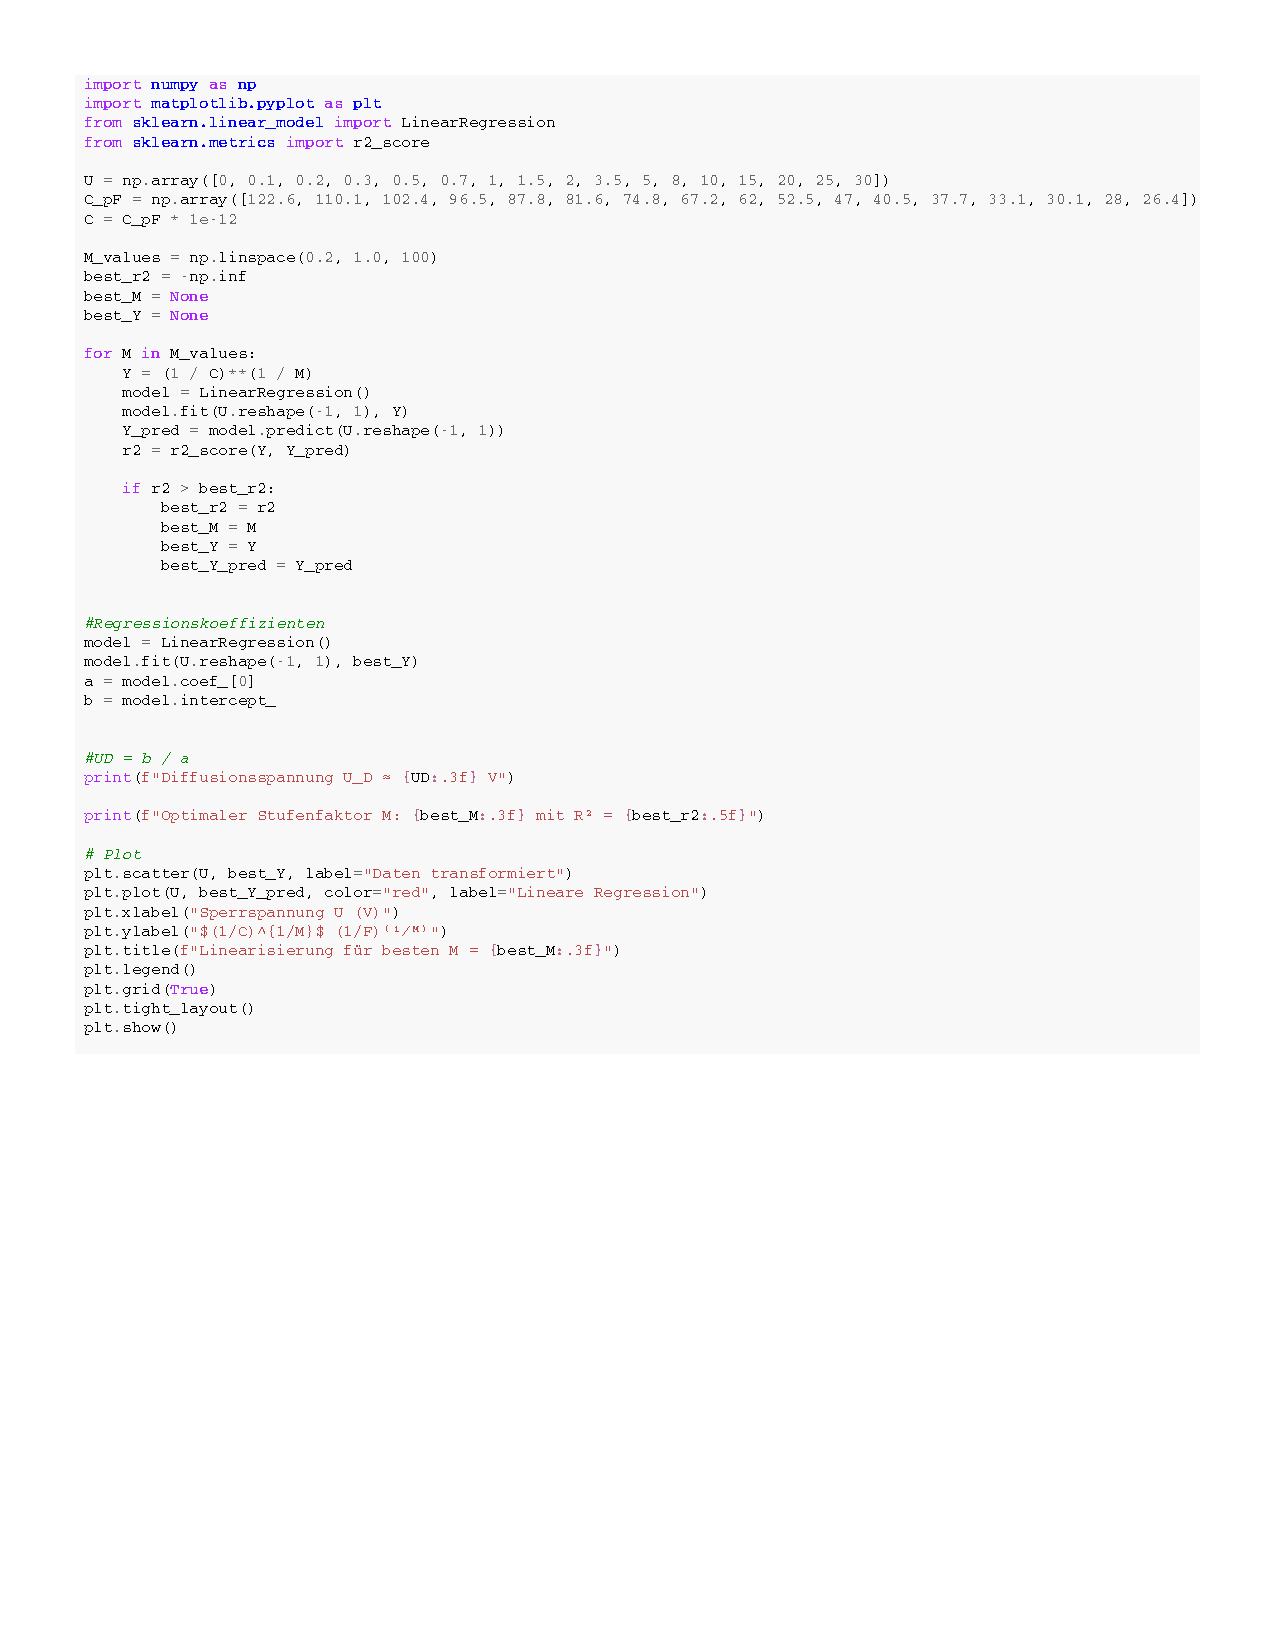
\includepdf[pages=-]{stufenfaktorskript.pdf}

\end{document}